% Options for packages loaded elsewhere
\PassOptionsToPackage{unicode}{hyperref}
\PassOptionsToPackage{hyphens}{url}
%
\documentclass[
]{book}
\usepackage{amsmath,amssymb}
\usepackage{lmodern}
\usepackage{ifxetex,ifluatex}
\ifnum 0\ifxetex 1\fi\ifluatex 1\fi=0 % if pdftex
  \usepackage[T1]{fontenc}
  \usepackage[utf8]{inputenc}
  \usepackage{textcomp} % provide euro and other symbols
\else % if luatex or xetex
  \usepackage{unicode-math}
  \defaultfontfeatures{Scale=MatchLowercase}
  \defaultfontfeatures[\rmfamily]{Ligatures=TeX,Scale=1}
\fi
% Use upquote if available, for straight quotes in verbatim environments
\IfFileExists{upquote.sty}{\usepackage{upquote}}{}
\IfFileExists{microtype.sty}{% use microtype if available
  \usepackage[]{microtype}
  \UseMicrotypeSet[protrusion]{basicmath} % disable protrusion for tt fonts
}{}
\makeatletter
\@ifundefined{KOMAClassName}{% if non-KOMA class
  \IfFileExists{parskip.sty}{%
    \usepackage{parskip}
  }{% else
    \setlength{\parindent}{0pt}
    \setlength{\parskip}{6pt plus 2pt minus 1pt}}
}{% if KOMA class
  \KOMAoptions{parskip=half}}
\makeatother
\usepackage{xcolor}
\IfFileExists{xurl.sty}{\usepackage{xurl}}{} % add URL line breaks if available
\IfFileExists{bookmark.sty}{\usepackage{bookmark}}{\usepackage{hyperref}}
\hypersetup{
  pdftitle={Modelación matemática},
  pdfauthor={Gerardo Martín},
  hidelinks,
  pdfcreator={LaTeX via pandoc}}
\urlstyle{same} % disable monospaced font for URLs
\usepackage{longtable,booktabs,array}
\usepackage{calc} % for calculating minipage widths
% Correct order of tables after \paragraph or \subparagraph
\usepackage{etoolbox}
\makeatletter
\patchcmd\longtable{\par}{\if@noskipsec\mbox{}\fi\par}{}{}
\makeatother
% Allow footnotes in longtable head/foot
\IfFileExists{footnotehyper.sty}{\usepackage{footnotehyper}}{\usepackage{footnote}}
\makesavenoteenv{longtable}
\usepackage{graphicx}
\makeatletter
\def\maxwidth{\ifdim\Gin@nat@width>\linewidth\linewidth\else\Gin@nat@width\fi}
\def\maxheight{\ifdim\Gin@nat@height>\textheight\textheight\else\Gin@nat@height\fi}
\makeatother
% Scale images if necessary, so that they will not overflow the page
% margins by default, and it is still possible to overwrite the defaults
% using explicit options in \includegraphics[width, height, ...]{}
\setkeys{Gin}{width=\maxwidth,height=\maxheight,keepaspectratio}
% Set default figure placement to htbp
\makeatletter
\def\fps@figure{htbp}
\makeatother
\setlength{\emergencystretch}{3em} % prevent overfull lines
\providecommand{\tightlist}{%
  \setlength{\itemsep}{0pt}\setlength{\parskip}{0pt}}
\setcounter{secnumdepth}{5}
\usepackage{booktabs}
\ifluatex
  \usepackage{selnolig}  % disable illegal ligatures
\fi
\usepackage[]{natbib}
\bibliographystyle{apalike}

\title{Modelación matemática}
\author{Gerardo Martín}
\date{2021-08-02}

\begin{document}
\maketitle

{
\setcounter{tocdepth}{1}
\tableofcontents
}
\hypertarget{preuxe1mbulo}{%
\chapter{Preámbulo}\label{preuxe1mbulo}}

\begin{center}
\includegraphics[width=20.83in]{logo} \end{center}

En el curso \textbf{Modelación matemática} aprenderemos a utilizar algunas herramientas matemáticas para analizar y entender los procesos de interés en ciencias ambientales. Los contenidos del índice se apegan al \href{Programa-curso.pdf}{programa completo del curso}, el cual se impartirá en los \href{Horario.pdf}{horarios normales establecidos}. Para conocer cuándo, cómo y qué temas se se impartirán puedes consultar la \href{Estrategia-docente.pdf}{estrategia docente}.

\hypertarget{criterios-de-evaluaciuxf3n}{%
\chapter{Criterios de evaluación}\label{criterios-de-evaluaciuxf3n}}

Las constribuciones a cada calificación parcial serán:

\begin{itemize}
\tightlist
\item
  Asistencia (25\%)
\item
  Trabajos de clase cumplidos (50\%)
\item
  Examen (25\%)
\item
  Participación (2 puntos extra máximo)
\end{itemize}

Cabe señalar, que la asistencia no corresponderá con su presencia en las sesiones sincrónicas, sino con el cumplimiento de los trabajos de clase. La participación se medirá tanto por participación directa en las sesiones sincrónicas como por el seguimiento que uds den a la clase por correo electrónico.

\hypertarget{unidad-i-modelos-determinuxedsticos}{%
\chapter{Unidad I: Modelos determinísticos}\label{unidad-i-modelos-determinuxedsticos}}

\hypertarget{introducciuxf3n-a-la-modelaciuxf3n}{%
\section{Introducción a la modelación}\label{introducciuxf3n-a-la-modelaciuxf3n}}

Imaginemos a seis personas invidentes, con la tarea de encontrar qué es el objeto que está frente a ellas usando únicamente el tacto. En la parábola de los seis hombres ciegos, el objeto es un elefante, de modo que la imágen que cada uno de ellos se forma del objeto depende enteramente de la parte del elefante que están tocando.

\begin{figure}

{\centering 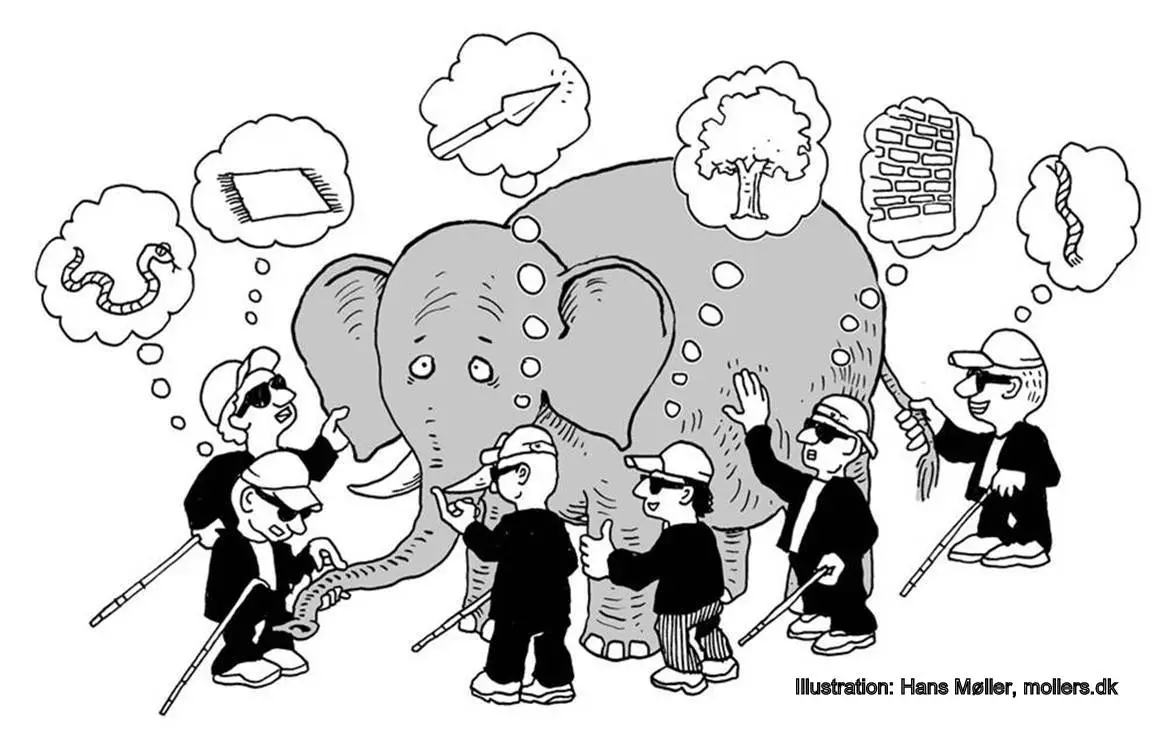
\includegraphics[width=16.17in]{Unidad-I/elefante} 

}

\caption{La parábola de los seis hombres ciegos inspeccionando un elefante.}\label{fig:unnamed-chunk-6}
\end{figure}

Quien toque los colmillos podrá pensar que se trata de una lanza, la trompa podría tratarse de una serpiente, la cola de una cuerda, las patas troncos de árbol y el cuerpo una pared. Es evidente que todas las hipótesis presentadas después de la inspección fueron erróneas, y que cuando estudiamos al mundo lo haremos igual, con la descripción de tan sólo una fracción de éste. Un séptimo hombre que pregunte a los otros seis qué fue lo que vieron podría formarse una imágen más completa del \emph{sistema} para proponer otra hipótesis: se trata de un objeto grande reposando sobre cuatro columnas con apéndices adelante y atrás.

Al estudiar los sistemas ecológicos, al igual que los ciegos, no sabremos que estamos frente a un elefante. Los sistemas ecológicos, al igual que los elefantes, también tienen componentes interconectados, y nosotros los ecólogos somos como los hombres ciegos, sólo podemos observar ciertas partes de los ecosistemas. En nuestro trabajo entonces, aprender a identificar y proponer hipótesis sobre cómo funcionan los sistemas ecológicos.

Las hipótesis propuestas por los seis hombres representan modelos, es decir simplificaciones del mundo que nos ayudan a entenderlo. Los modelos matemáticos son simplificaciones formales del mundo utilizando otro lenguaje, las matemáticas.

\hypertarget{funciones-buxe1sicas-y-su-representaciuxf3n-en-el-plano-cartesiano}{%
\section{Funciones básicas y su representación en el plano cartesiano}\label{funciones-buxe1sicas-y-su-representaciuxf3n-en-el-plano-cartesiano}}

\hypertarget{la-luxednea-recta}{%
\subsection{La línea recta}\label{la-luxednea-recta}}

Una línea recta se puede representar matemáticamente de varias maneras, la más común de ellas es por medio de una función. Una función, en cambio es una expresión matemática que indica una serie de operaciones (aritméticas por ejemplo), que serán aplicadas a un conjunto de números en sucesión (los números reales, p.~ej.) para producir otro conjunto. Así la, función lineal más sencilla puede ser:

\begin{equation}
    y(x) = x
\end{equation}

Lo que quiere decir que \(y\) es una función de \(x\), y cada valor de \(y\) será igual a cada valor de \(x\). En lenguaje matemático, el conjunto de números de \(x\) se llama el dominio, y \(y(x)\) el codominio. Algunas funciones lineales más complejas son:

\begin{equation}
    y(x) = ax
\end{equation}

donde \(a\) es una constante, lo que quiere decir que cada valor de \(y(x)\) será producido por el producto \(a \times x\). Finalmente, la expresión más común de una ecuación lineal es:

\begin{equation}
    y(x) = b + ax
\end{equation}

donde \(b\) también es una constante que se llama intercepto, y \(a\) es la pendiente, pues esta última determina la inclinación de la línea recta representada en el plano cartesiano.

\hypertarget{representaciones-gruxe1ficas-de-la-recta}{%
\subsubsection{Representaciones gráficas de la recta}\label{representaciones-gruxe1ficas-de-la-recta}}

Comencemos por dar un repaso del plano cartesiano. Este consiste de la representación de dos conjuntos de números reales en los que representamos una función, como una regla de correspondencia entre los valores de cada conjunto, de modo que a cada valor de \(x\) corresponde uno y sólo uno de los valores de \(y\). Cada conjunto se puede representar como una recta, y cuando éstas se disponen perperdiculares dan origen al plano.

\begin{figure}

{\centering 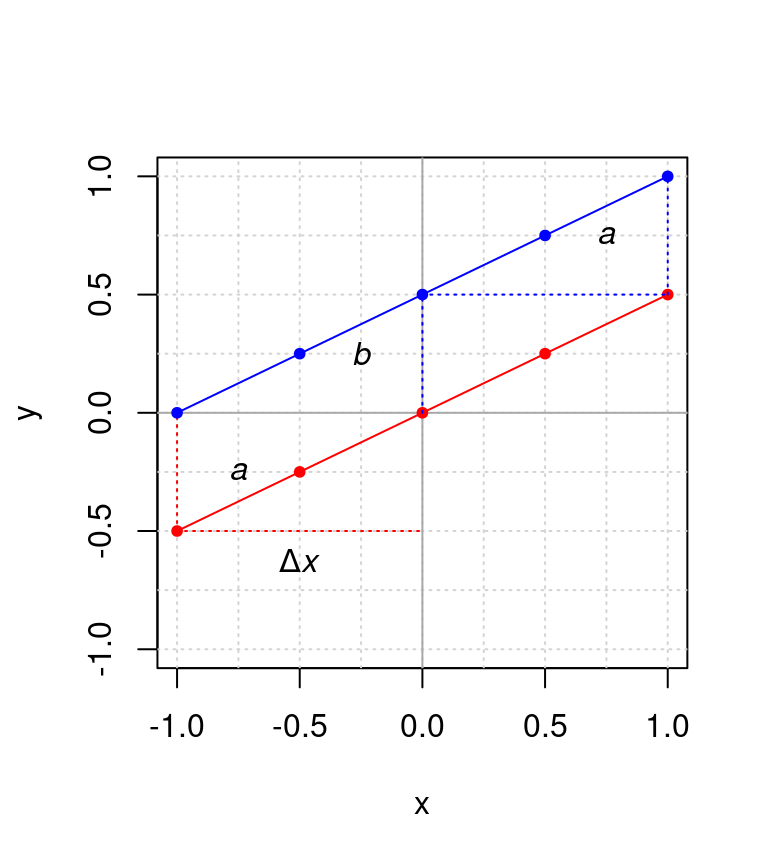
\includegraphics{Model-mate_files/figure-latex/unnamed-chunk-7-1} 

}

\caption{Ejemplo del plano cartesiado mostrando en rojo la correspondencia de valores para $y(x) = x$, donde los puntos corresponden a los pares de valores $(x = -1, y = -1), (-0.5, -0.5), (0, 0), (0.5, 0.5), (1, 1)$.}\label{fig:unnamed-chunk-7}
\end{figure}

Ahora veamos, con un ejemplo gráfico por qué la constante \(a\) recibe el nombre de \emph{pendiente}.

\begin{figure}

{\centering 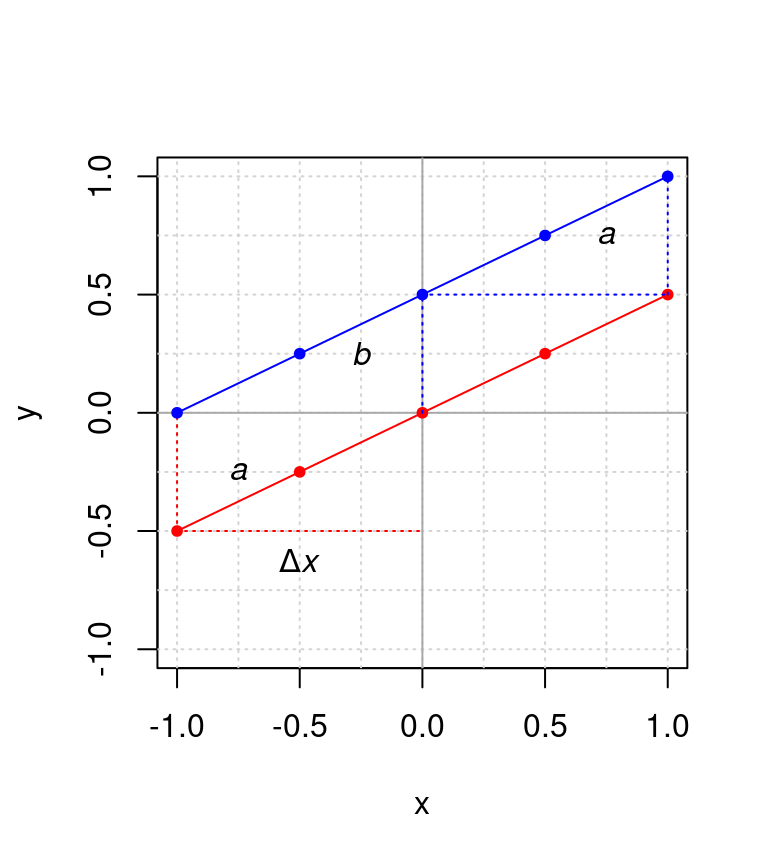
\includegraphics{Model-mate_files/figure-latex/unnamed-chunk-8-1} 

}

\caption{Gráficas de las funciones $y(x) = 0.5 x$ (en rojo) y $y(x) = 0.5 + 0.5 x$ (azul). Las líneas punteadas en colores indican el efecto de las constantes $a$ y $b$, mientas que Δ$x$ denota el cambio de una unidad de $x$.}\label{fig:unnamed-chunk-8}
\end{figure}

Como podemos ver, de manera más general, la línea recta es generada por una regla de correspondencia muy sencilla, un conjunto de valores \(X\) son multiplicados por un escalar \(a\), a los que se les puede añadir un \emph{intercepto} \(b\). El intercepto siempre es el valor de \(y(x)\) cuando \(x = 0\).

Ya se podrán imaginar que puede existir un sinnúmero de modelos lineales distintos, por ejemplo si \(y\) es una función de un gran número de conjuntos \(X\):

\begin{equation}
y(x_1, x_2, \dots, x_{n-1}, x_n) = b + a_1 x_1 + a_2 x_2 + \dots + a_{n-1} x_{n-1} + a_n x_n
\end{equation}

Gráficamente, estamos prácticamente limitados a explorar \(y(x_1, x_2)\), pero existen muchas herramientas matemáticas para entender modelos lineales más complejos que veremos más adelante. Estas herramientas y las implicaciones generales de la simplicidad del modelo lineal lo hacen uno de los modelos más útiles con que contamos para estudiar matemáticamente fenómenos dinámicos (que cambian de estado a lo largo del tiempo), como para estudiarlos de manera probabilística (con estadística). De hecho, el modelo lineal nos puede servir para entender modelos, como la parábola y el exponencial, que geométricamente no se parecen a la línea recta.

\hypertarget{la-paruxe1bola}{%
\subsection{La parábola}\label{la-paruxe1bola}}

Geométricamente, la parábola es muy distinta de la recta:

\begin{figure}

{\centering 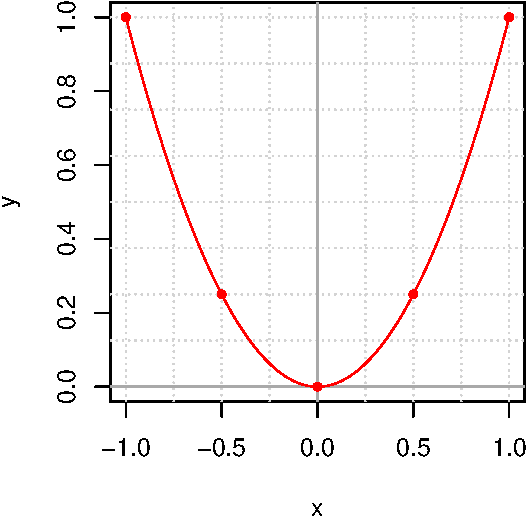
\includegraphics{Model-mate_files/figure-latex/parabola-1} 

}

\caption{Ejemplo del plano cartesiado mostrando en rojo la correspondencia de valores para $y(x) = x^2$, donde los puntos corresponden a los pares de valores $(x = -1, y = 1), (-0.5, 0.25), (0, 0), (0.5, 0.25), (1, 1)$.}\label{fig:parabola}
\end{figure}

La función matemática más sencilla que puede describir esta forma en el plano cartesiano es:

\begin{equation}
    y(x) = x^2
\end{equation}

Al igual que con los modelos lineales, las parábolas pueden representarse matemáticamente de otras formas más complejas:

\begin{itemize}
\tightlist
\item
  \(y(x) = a + bx + cx^2\)
\item
  \(y(x) = a + cx^2\)
\item
  \(y(x) = -x^2\)
\end{itemize}

Si uno es observador, se dará cuenta de que estas ecuaciones son muy similares a la recta, y es que es posible considerar que \(x^2\) se puede considerar como otro conjunto tal que \(x' = x^2\), resultando así en funciones perferctamente lineales:

\begin{itemize}
\tightlist
\item
  \(y(x) = a + bx + cx'\)
\item
  \(y(x) = a + cx'\)
\item
  \(y(x) = -x'\)
\end{itemize}

Entonce, lo que realmente distingue matemáticamente a una parábola de una recta, es la doble ocurrencia de cada valor de \(y\) para los distintos valores de \(x\):

\begin{figure}

{\centering 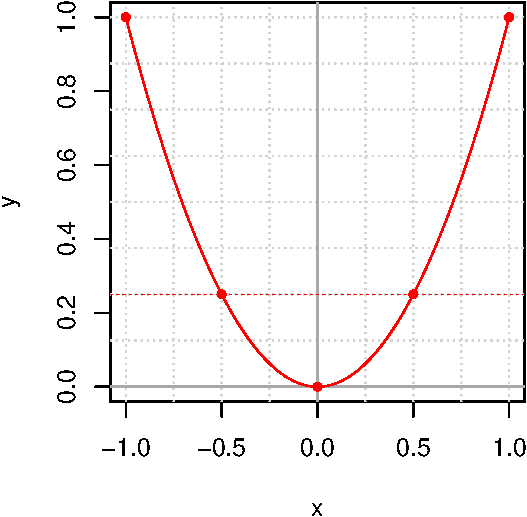
\includegraphics{Model-mate_files/figure-latex/parabola-2-1} 

}

\caption{Correspondencia de dos valores distintos de $x$ para el mismo valor de $y$}\label{fig:parabola-2}
\end{figure}

Cuando esto ocurre, las funciones tiene un solo punto a lo largo de todos los valores de \(x\), donde sólo va a ocurrir un valor único de \(y\). A estos puntos se les conocen como mínimos (par de valores con coordenadas \((0, 0)\) en la figura \ref{fig:parabola-2}). Los máximos, en cambio están ilustrados en la figura \ref{fig:parabola-3}.

\begin{figure}

{\centering 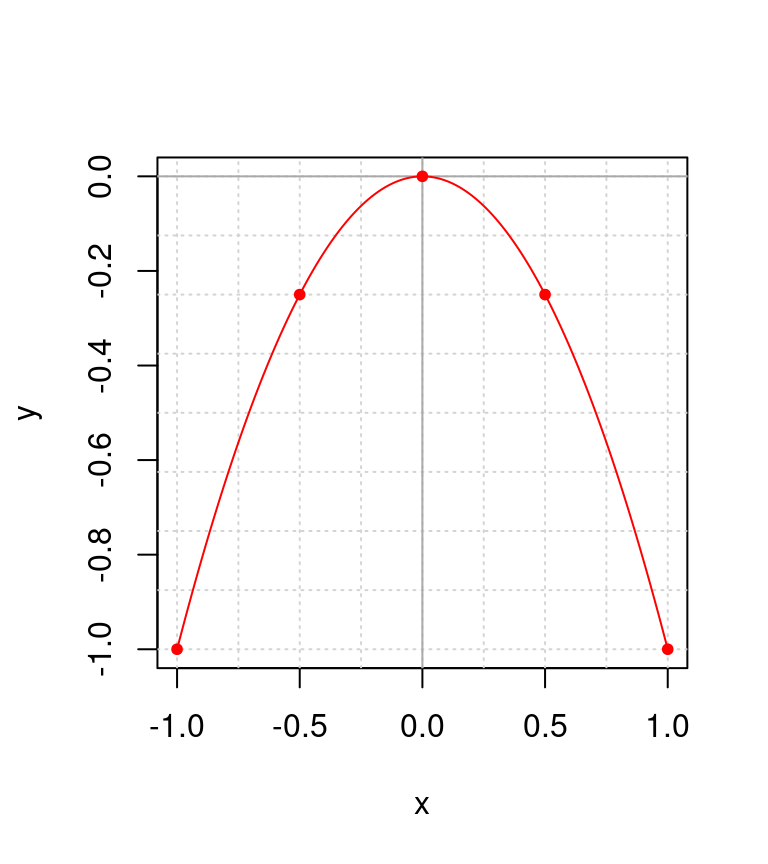
\includegraphics{Model-mate_files/figure-latex/parabola-3-1} 

}

\caption{Correspondencia de valores para $y = -x^2$.}\label{fig:parabola-3}
\end{figure}

\hypertarget{funciones-complementarias-y-su-representaciuxf3n-en-dos-y-tres-dimensiones}{%
\section{Funciones complementarias y su representación en dos y tres dimensiones}\label{funciones-complementarias-y-su-representaciuxf3n-en-dos-y-tres-dimensiones}}

\hypertarget{la-luxednea-recta-como-modelo-universal}{%
\section{La línea recta como modelo ``universal''}\label{la-luxednea-recta-como-modelo-universal}}

\hypertarget{modelaciuxf3n-de-sistemas-sociales-y-ambientales}{%
\section{Modelación de sistemas sociales y ambientales}\label{modelaciuxf3n-de-sistemas-sociales-y-ambientales}}

\hypertarget{methods}{%
\chapter{Methods}\label{methods}}

We describe our methods in this chapter.

\hypertarget{applications}{%
\chapter{Applications}\label{applications}}

Some \emph{significant} applications are demonstrated in this chapter.

\hypertarget{example-one}{%
\section{Example one}\label{example-one}}

\hypertarget{example-two}{%
\section{Example two}\label{example-two}}

  \bibliography{book.bib,packages.bib}

\end{document}
